\documentclass[11pt, a4paper]{article} 
\usepackage[polish]{babel}
\usepackage{longtable}
\usepackage{booktabs}
\usepackage{dcolumn}
\usepackage{geometry} % to change the page dimensions
\usepackage{graphicx} % support the \includegraphics command and options
\usepackage{float}
\usepackage{array} % for better arrays (eg matrices) in maths
\usepackage{verbatim} % adds environment for commenting out blocks of text & for better verbatim
\usepackage{lscape}
\usepackage{latexsym}
\usepackage{multirow}
\usepackage{amsmath}
\usepackage{makecell}
\let\lll=\amslll
%\savesymbol{lll}
\usepackage{amssymb}
\usepackage{enumerate}
\usepackage{pdflscape} 
\usepackage{epstopdf}
\usepackage{pdfpages}


\usepackage{fontspec}
%\usepackage[OT4]{fontenc}
%\usepackage[utf8]{inputenc}


\setlength\parindent{0pt}

\newcommand{\HRule}{\rule{\linewidth}{0.5mm}}
\newcommand{\linia}{\rule{\linewidth}{0.1mm}}
\usepackage[  
  bookmarks=true,  
  bookmarksnumbered=false,  
  unicode=true,  
  pdftitle={Projekt zespołowy},
  pdfauthor={Paweł Bogner, Krzysztof Nomejko, Grzegorz Maj,
  Bartosz Folta, Marcin Dmochowski},
  pdfnewwindow=true,
  colorlinks=true,
  citecolor=black,
  urlcolor=black,
  filecolor=black,
  linkcolor=black
]{hyperref} 

\begin{document}
	%%%%%%%%%%%%%%%%%%%%%%%%%%%%%%%%%%%
% Strona tytułowa
%\newcommand{\HRule}{\rule{\linewidth}{0.5mm}}
\begin{titlepage}
  \begin{center}
    
    % Upper part of the page
    %\centering{\includegraphics[width=0.2\textwidth]{logo.png}\\[1cm]}

    \textsc{\Large Systemy zdarzeniowe}\\[3cm]
    
    % Title
    \centering{\HRule \\[0.5cm]}
	      {\LARGE  \textsc{Raport}\\[0.4cm]}
	      {\Large Opracowanie rozproszonego systemu koordnacji
                agentów mobilnych}
	      \centering{\HRule \\[1.5cm]}
	      
	      % Autor i prowadzący
	      \begin{minipage}{0.4\textwidth}
	        \begin{flushleft} \large
	          \emph{Skład grupy:}\\
	          Paweł \textsc{Bogner} \\
	          Marcin \textsc{Dmochowski} \\
	          Bartosz \textsc{Folta} \\	
	          Grzegorz \textsc{Maj} \\
	          Krzysztof \textsc{Nomejko} \\
		  
		  
	        \end{flushleft}
	      \end{minipage}
	      \begin{minipage}[b]{0.4\textwidth}
	        \begin{flushright} \large
		  \emph{Prowadzący:} \\
		  dr~inż. E.~\textsc{Roszkowska}
	        \end{flushright}

	      \end{minipage}
	      \vfill
	      % Bottom of the page
	          {\large \today}

  \end{center}
\end{titlepage}
%%%%%%%%%%%%%%%%%%%%%%%%%%%%%%%%%%%

	
	\noindent Zdecydowano, że zostanie wykorzystana tradycyjna, płaska struktura
zarządzania z jednym liderem (koordynatorem).  Do zadań lidera należy
podejmowanie krytycznych decyzji projektowych, rozstrzyganie sporów
oraz kontrolowanie postępu prac nad przydzielonymi zadaniami.
\\\\
\noindent W kwestii rozstrzygania sporów, strona konfliktu ma prawo do
przedstawienia problemu na forum grupy, w celu jego wspólnego
przedyskutowania.  W świetle przedstawionych argumentów i poglądów
lider ma obowiązek podjąć decyzję rozstrzygającą.
\\\\
\noindent Za termin regularnych spotkań przyjęto termin zajęć odbywających się w
ramach kursu ,,Systemy zdarzeniowe''. Lider zespołu ma prawo
zarządzenia dodatkowego spotkania organizacyjnego na wniosek jednego
lub kilku członków zespołu.  Osoba wnosząca o zorganizowanie zebrania
ma obowiązek wykazać, że spotkanie jest niezbędne w celu dalszego
rozwoju projektu.
\\\\
\noindent Do przewidzianych środków komunikacji zdalnej należą ,,Google
groups'', ,,Redmine'' oraz rozmowy telefoniczne.  W celu składowania i
wymiany dokumentów zostanie wykorzystane oprogramowanie ,,SVN''.
Każdy z członków grupy na obowiązek korzystać z tego programu.  Jako
mechanizm monitorowania postępów prac zostanie wykorzystana usługa
,,Redmine''.  Jest to narzędzie, które pozwala przydzielić zadanie
danemu członkowi lub członkom zespołu, określić ramy czasowe jego
wykonania, oraz śledzić postęp prac.
\\\\
\noindent Uznano, że każdy członek grupy zostanie obdarzony prawami własności
intelektualnej do części projektu, za której zrealizowanie był
odpowiedzialny.


%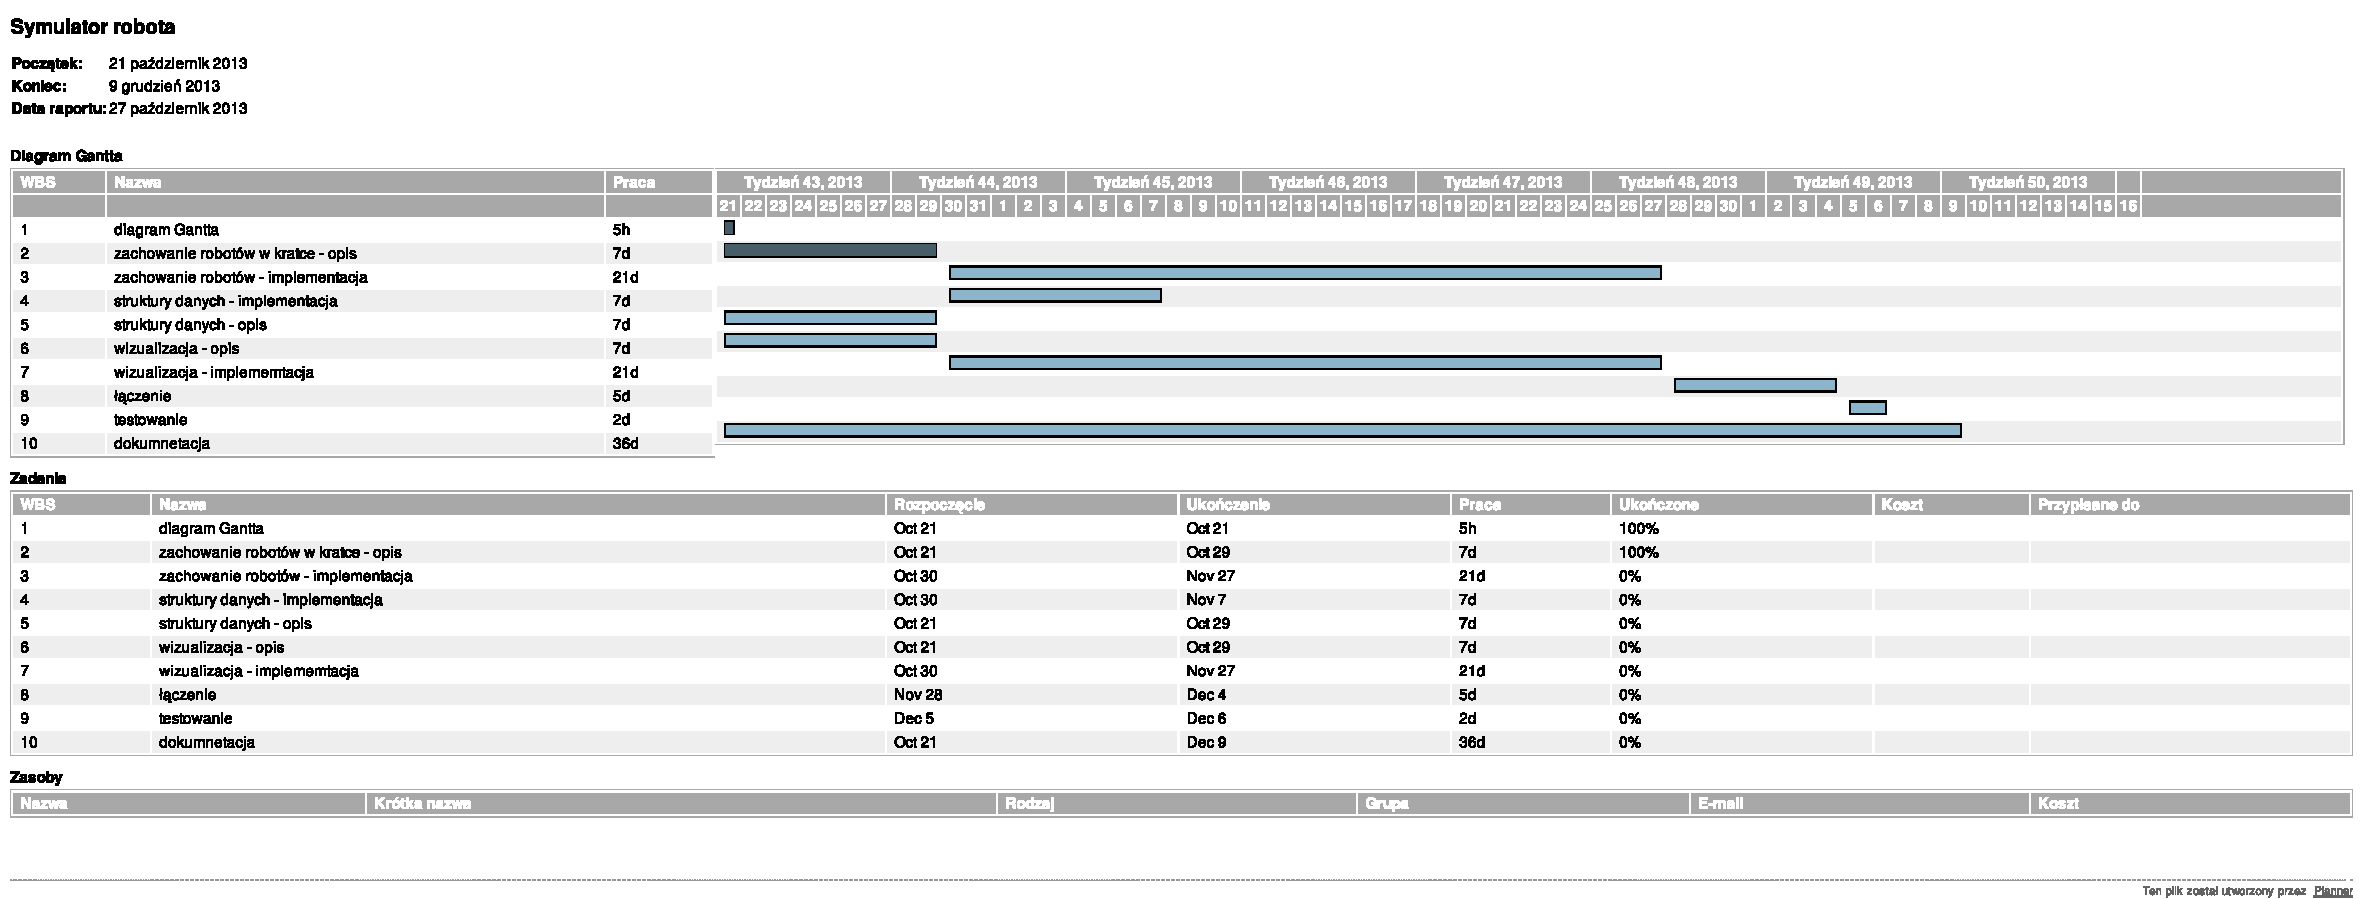
\includepdf[landscape]{img/gantt.pdf}

	\section{Opis logiki}

Działania w systemie są odpowiedzią na zdarzenia wynikające z komunikacji serwer-symulator.

\begin{enumerate}
  \item pobranie informacji początkowych od serwera: współrzędne
    sektora początkowego,

  \item wysłanie zapytania o pozwolenie wjazdu do kolejnego
    sektora, \label{zapytanie}

  \item oczekiwanie na pozwolenie, przy jednoczesnym poruszaniu się
    zgodnie z wektorem wyznaczonym przez pola potencjałów,
    
  \item otrzymanie pozwolenia na wjazd do kolejnego sektora,
    ustawienie przeciwnego potencjału na ścianie sąsiadującej z
    kolejnym sektorem, otrzymanie współrzędnych następnego sektora
    docelowego,

  \item przejazd do kolejnego sektora,

  \item zwolnienie poprzedniego sektora, przejście do punktu \ref{zapytanie}.

\end{enumerate}





	\section{Zachowanie robotów wewnątrz pola}
	Zachowanie robotów wewnątrz pola zamodelowane jest za pomocą metody sztucznych pól potencjałów. Potencjały ustalane są w następujący sposób:
	\begin{itemize}
		\item robot oczekujący na zezwolenie wyjazdu z pola widzi wszystkie ściany jako spolaryzowane ładunkiem o znaku zgodnym ze znakiem jego ładunku (rys. \ref{pic:waiting}), a jego wektor sił ma składowe opisane następującymi równaniami:
                  $$F_x= A((X-x)^2 - x^2)$$
                  $$F_y= A((Y-y)^2 - y^2),$$
		\item robot wykonujący manewr przejazdu do innego pola widzi dodatkowy ładunek na ścianie, w kierunku której ma zmierzać (umieszczony z jej prawej strony, aby zapobiegać kolizjom) (rys. \ref{pic:moving}), a do składowych jego wektora sił dodaje się człon odpowiedzialny za modelowanie dodatkowego potencjału:
                  $$F_{xM}= +B(X_p-x)^2$$
                  $$F_{yM}= +B(Y_p-y)^2,$$
		\item dwa roboty znajdujące się w tym samym polu zawsze są spolaryzowane ładunkami punktowymi o jednakowych znakach (rys. \ref{pic:tworobots}), a do wektora sił dodawany jest w tym wypadku następujący człon modelujący siłę wzajemnie je odpychającą:
                  $$F_{xD}= +C(x-x_D)^2$$
                  $$F_{yD}= +C(y-y_D)^2,$$ 
		\item w wypadku, jeśli w polu znajdują się dwa roboty, każdy widzi inną polaryzację ścian -- taką, aby zgadzała się ona z jego stanem ruchu (oczekiwanie, zezwolenie na przejazd),
                \item przykład --- kiedy w polu znajdują się dwa roboty i robot, dla którego obliczamy wypadkowy wektor sił, wyjeżdża z pola, składowe jego sił opisane są nastepującymi równaniami:
                  $$F_x= A((X-x)^2 - x^2)+B(X_p-x)^2+C(x-x_D)^2$$
                  $$F_y= A((Y-y)^2 - y^2)+B(Y_p-y)^2+C(y-y_D)^2.$$ 
	\end{itemize}
	
	\begin{figure}[H]
		\centering
		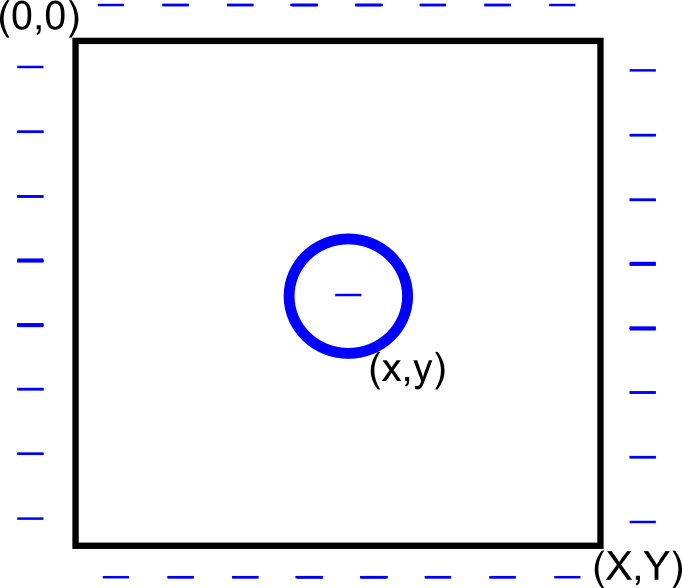
\includegraphics[scale=0.9]{img/waiting.png}
		\caption{Robot oczekujący na pozwolenie na wyjazd z komórki}
		\label{pic:waiting}
	\end{figure}
	\begin{figure}[H]
		\centering
		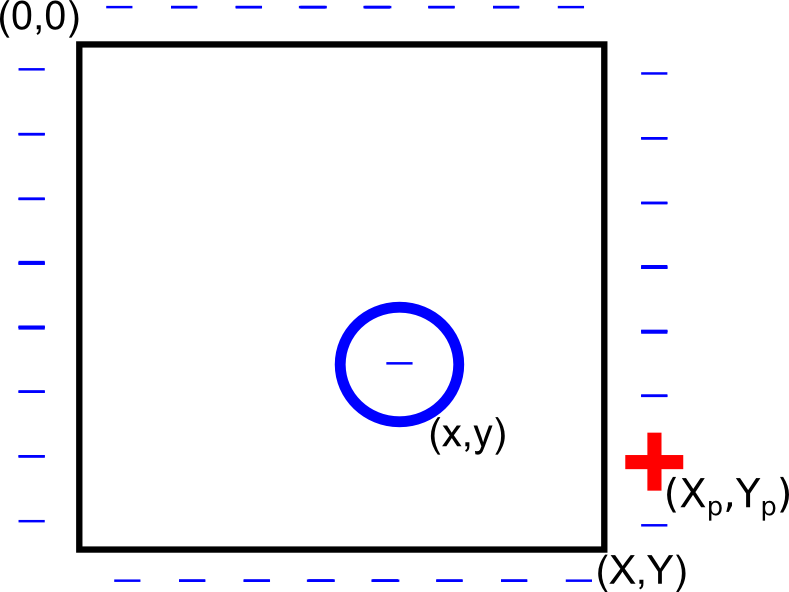
\includegraphics[scale=0.9]{img/moving.png}
		\caption{Robot wyjeżdżający z komórki}
		\label{pic:moving}
	\end{figure}
	\begin{figure}[H]
		\centering
		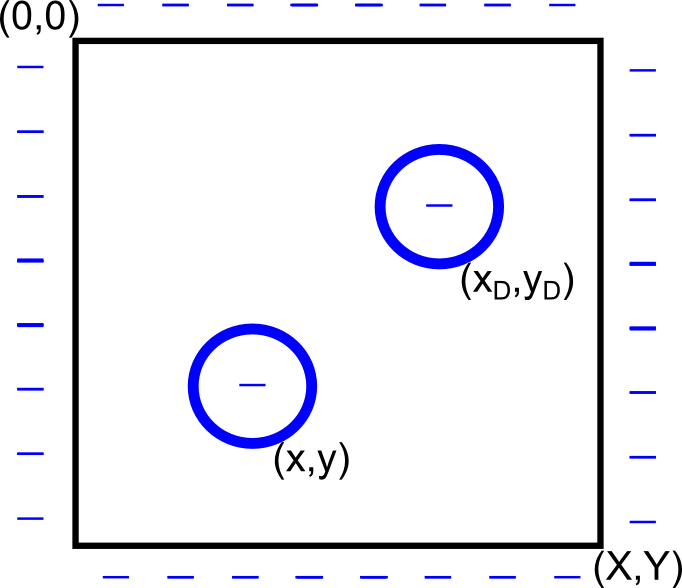
\includegraphics[scale=0.9]{img/tworobots.png}
		\caption{Dwa roboty oczekujące na pozwolenie na wyjazd z pola}
		\label{pic:tworobots}
	\end{figure}

	
\section{Zarys struktur danych}
\subsection{Scena}
W zaproponowanym modelu scena (plansza) jest strukturą, zawierającą tablicę komórek, a także ewentualne informacje związane z modelem robota wspólne dla wszystkich. Pojedyncza komórka zawierałaby informacje o swoich wymiarach oraz listę robotów, które aktualnie się w niej znajdują, a także wskaźnik do struktury zawierającej modele dla metody pól potencjałów.
\subsection{Dane wymieniane z serwerem}
Serwer ma zadanie planowania tras dla robotów, wobec czego pożądana informacja dla każdego z robotów to następna komórka, do której ten ma się kierować oraz zezwolenie bądź brak zezwolenia na wjazd do niej. W przypadku braku zezwolenia robot zatrzymałby się w bieżącej komórce; w przeciwnym wypadku przejechałby od razu do następnej komórki.\\\\Klient miałby za zadanie wysyłania zapytań o dalsze drogi robotów oraz o pozwolenie na ich realizację, a także informowałby o wykonanych zadaniach i zjeździe robotów ze sceny.

	\section{Protokół komunikacji z serwerem}
Protokół komunikacji jest identyczny z zaimplementowanym w zalążku przez Adama Klamę. Opiera się on na transmisji pakietów danych o odpowiednich nagłówkach poprzez protokół TCP/IP. Wszystkie przekazywane wartości liczbowe mają typ danych int32\_t (czterobajtowy \textit{signed integer}).\\

Przebieg komunikacji z serwerem po uruchomieniu aplikacji:
\begin{enumerate}
\item Klient podłącza się do serwera.
\item\label{pkt:rejestracjarobota} Klient wysyła do serwera żądanie rejestracji robota:
\begin{itemize}
\item ramka zapytania ma rozmiar 8 bajtów oraz nagłówek oznaczony 1 (\texttt{REGISTER\_ROBOT}), zawiera ona kolejno lokalne id robota (id w kliencie) oraz promień robota;
\item ramka odpowiedzi ma rozmiar 24 bajty oraz nagłówek oznaczony 2 (\texttt{REGISTER\_ROBOT\_RESP}), zawiera ona kolejno globalne id robota (w serwerze), lokalne id robota (w kliencie), rozmiar pojedynczej komórki planszy w osi X, rozmiar pojedynczej komórki planszy w osi Y, liczba komórek planszy w osi X, liczba komórek planszy w osi Y.
\end{itemize}
\item\label{pkt:currentpos} Klient wysyła do serwera informację o początkowym położeniu właśnie zarejestrowanego robota:
\begin{itemize}
\item ramka zapytania ma rozmiar 12 bajtów oraz nagłówek oznaczony 6 (\texttt{CURRENT\_POSITION}), zawiera ona kolejno globalne id robota, położenie robota w osi X (tj. numer komórki, w której robot się znajduje, patrząc względem osi X), położenie robota w osi Y;
\item serwer nie odpowiada na to zapytanie.
\end{itemize}
\vspace{10pt}
Zdarzenia \ref{pkt:rejestracjarobota}, \ref{pkt:currentpos} powtarzają się tyle razy, ile dostępnych jest robotów, natomiast po zarejestrowaniu pierwszego robota serwer może przejść do wykonywania zdarzenia \ref{pkt:goto}.
\vspace{10pt}
\item\label{pkt:goto} Serwer wysyła robotowi, wybranemu spośród już zarejestrowanych, polecenie przejechania do jednej z sąsiednich komórek oraz sygnał, czy ma pozwolenie na przejazd do docelowej komórki:
\begin{itemize}
\item ramka zapytania ma rozmiar 28 bajtów oraz nagłówek oznaczony 4 (\texttt{RESPONSE\_SECTOR}), zawiera ona kolejno globalne id robota, docelowe położenie robota w osi X, docelowe położenie robota w osi Y, flaga oznaczająca pozwolenie na przejazd (1) lub też jego brak (0), numer klienta (w tej chwili ignorowany), docelowe położenie w osi X, docelowe położenie w osi Y;
\item klient nie odpowiada na to zapytanie.
\end{itemize}
\item\begin{enumerate}[a)]\item W przypadku braku pozwolenia na przejazd robot czeka na otrzymanie pozwolenia od serwera, przy czym zadaniem serwera jest monitorowanie faktu, że istnieje robot, który pytał o pozwolenie, dostał odmowę i znajduje się w stanie oczekiwania.
\item W przypadku otrzymania pozwolenia na przejazd robot przejeżdża do komórki docelowej i w momencie opuszczenia poprzedniej komórki całą swoją powierzchnią informuje serwer o zwolnieniu tejże:
\begin{itemize}
\item ramka zapytania ma rozmiar 16 bajtów oraz nagłówek oznaczony 3 (\texttt{REQUEST\_SECTOR}), zawiera ona kolejno globalne id robota, poprzednie położenie robota w osi X, poprzednie położenie robota w osi Y, flaga oznaczająca opuszczenie poprzedniej komórki - wartość liczbowa 0;
\item serwer nie odpowiada na to zapytanie.
\end{itemize}
\end{enumerate}
\end{enumerate}
	\section{Interfejs graficzny}
W celu stworzenia GUI wykorzystano biblioteki \textit{Qt}. Interfejs graficzny zosta� zaprojektowany z wykorzystaniem programu \textit{QtDesigner}.

\subsection{Wykorzystane klasy}
Tworz�c interfejs wykorzystano biblioteki:

\begin{itemize}
\item \textbf{QGraphicsScene} - biblioteka pozwalaj�ca na stworzenie obiektu reprezentuj�cego dwuwymiarow� scen� graficzn�, na scenie mo�na tworzy� i umieszcza� obiekty (pojedyncze piksele, wieloboki), obiekty mo�na poddawa� transformacji przy pomocy klasy \textit{QTransform},
\item \textbf{QGraphicsView} - biblioteka, przy pomocy kt�rej mo�na wizualizowa� zawarto�� sceny utworzonej z wykorzystaniem klasy \textit{QGraphicsScene}.
 \end{itemize}

\subsection{Proponowany interfejs}
\begin{figure}[H]
  \centering
  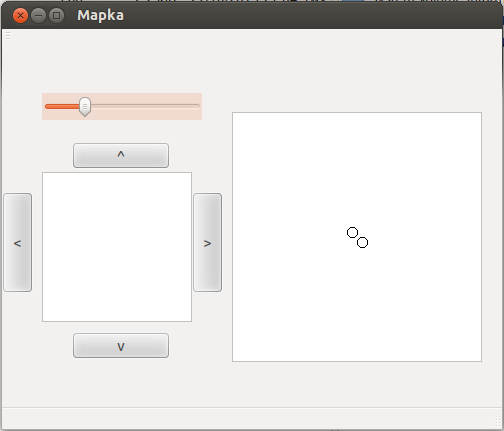
\includegraphics[width=0.5\textwidth]{img/okno.png}
\end{figure}




	\section{Zespół}
		\subsection*{Paweł Bogner}
			\begin{figure}[H]
	\centering
	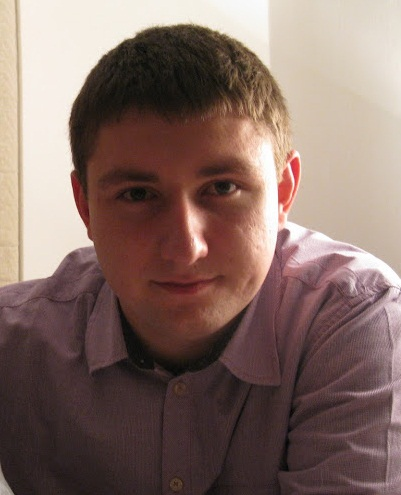
\includegraphics[width=0.4\textwidth]{img/pawel.jpg}
\end{figure}
Interesuje się elektroniką od strony sprzętowej, szczególnie systemami mikroprocesorowymi. Jego hobby to astronomia.\\
\textbf{Wynik testu Belbina: },,Racjonalny Analityk''

		\subsection*{Marcin Dmochowski}
			\begin{figure}[H]
	\centering
	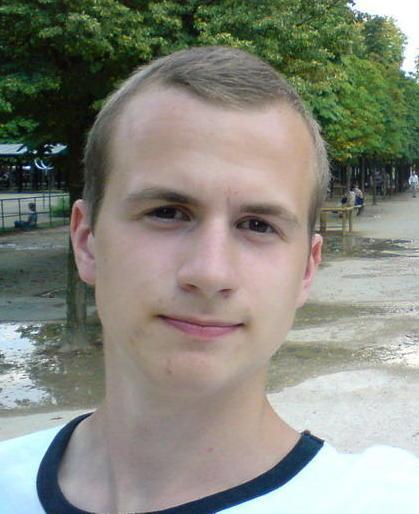
\includegraphics[width=0.35\textwidth]{img/marcin.jpg}
\end{figure}
Najbardziej upodoba� sobie zadania natury praktycznej i programowanie. Spo�r�d rzeczy niezwi�zanych z nauk� lubi tenis sto�owy i ziemny, bryd�, sporty zimowe i wodne, dobry film i ksi��k� oraz szachy.\\
\textbf{Wynik testu Belbina: },,Ambitny Komendant''

		\subsection*{Bartosz Folta}
			\begin{figure}[H]
	\centering
	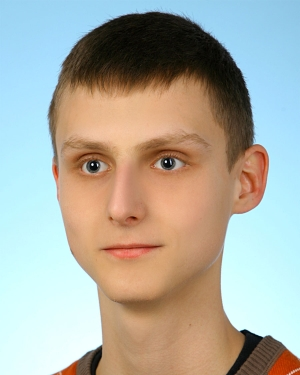
\includegraphics[width=0.4\textwidth]{img/bartek.jpg}
\end{figure}
Stara się rozwiązać spory drogą dyplomatyczną. Pozytywnie nastawiony do zadań wymagających doszkolenia się w danej dziedzinie. \\
\textbf{Wynik testu Belbina: },,dusza zespołu''

		\subsection*{Grzegorz Maj}
			\begin{figure}[H]
	\centering
	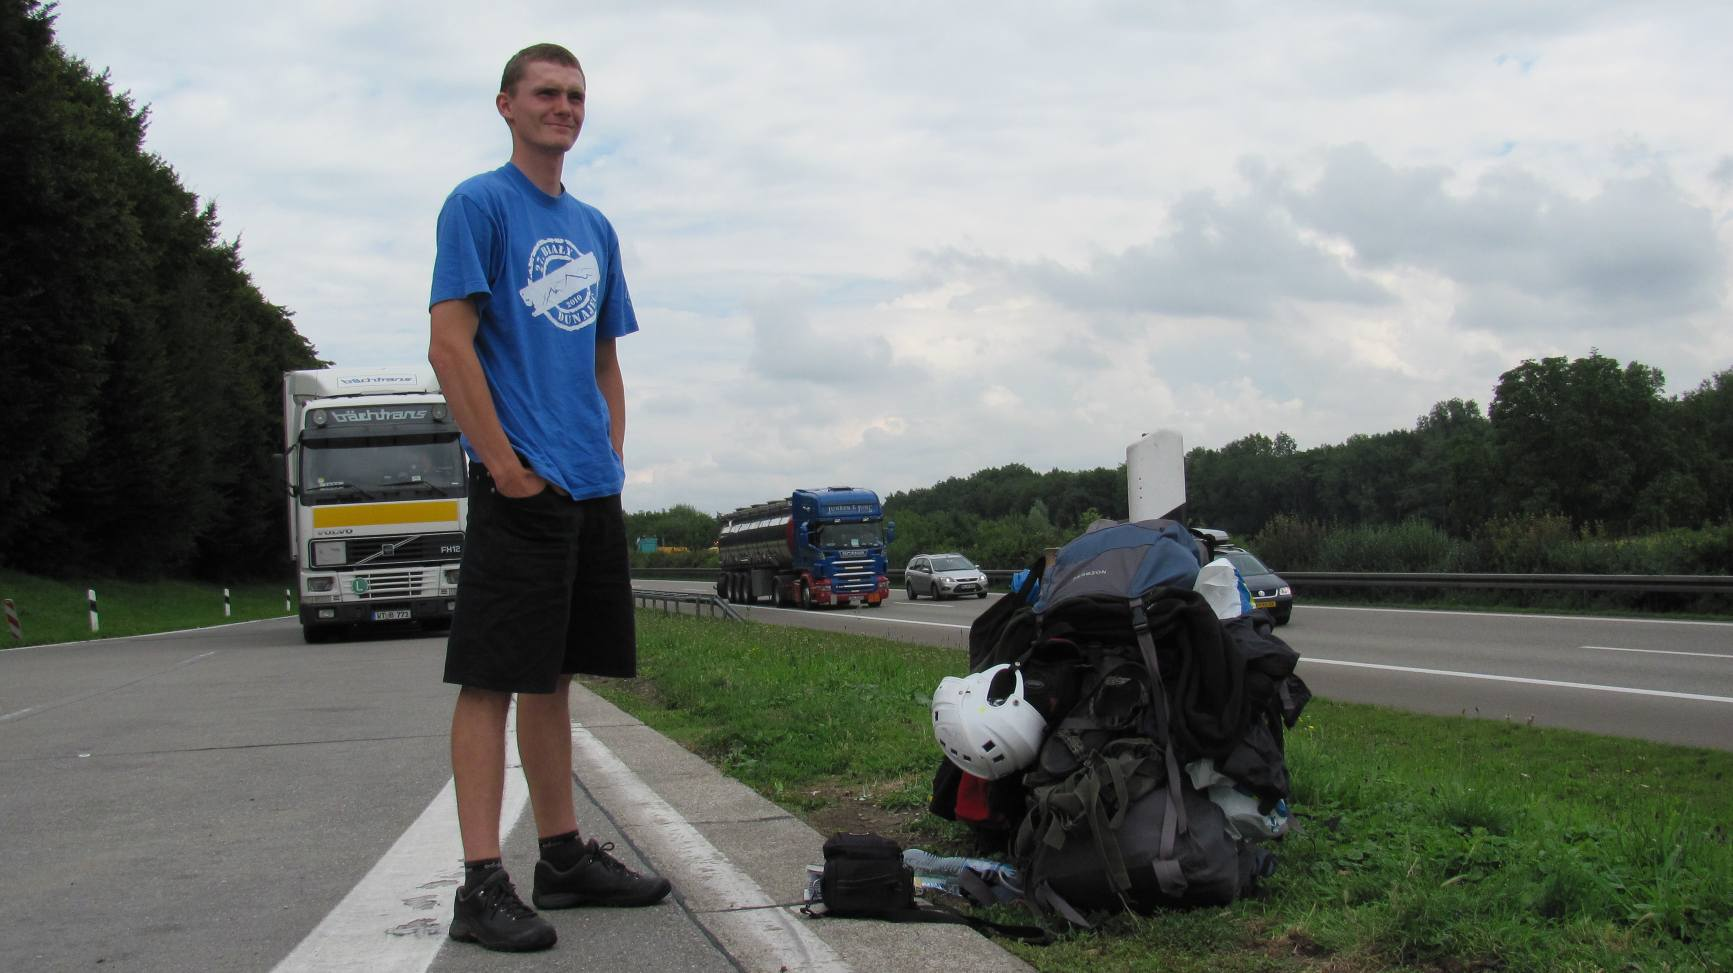
\includegraphics[width=0.4\textwidth]{img/grzesiek.jpg}
\end{figure}
Zainteresowania: g�ry, w szczeg�lno�ci wspinaczka i skitouring.\\
\textbf{Wynik testu Belbina: },,Racjonalny Analityk''


		\subsection*{Krzysztof Nomejko}
			\begin{figure}[H]
	\centering
	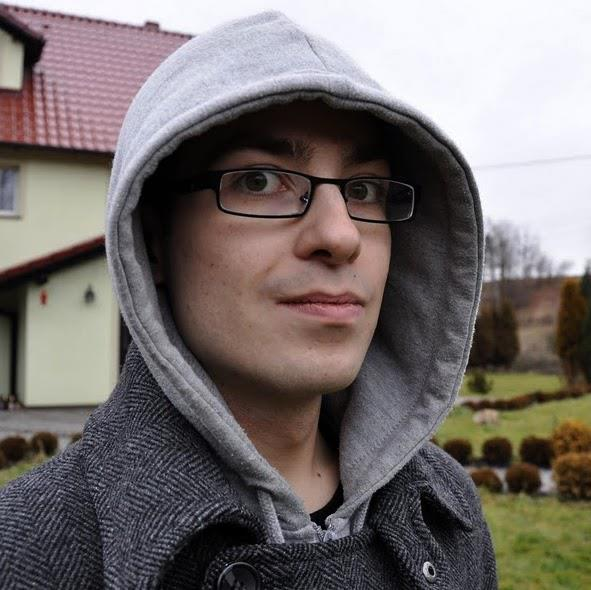
\includegraphics[width=0.4\textwidth]{img/krzysztof.jpg}
\end{figure}
Nieoceniony w ka�dej grupie. Bardziej praktyk ni� teoretyk.\\
\textbf{Wynik testu Belbina: },,Dusza Zespo�u''

\end{document}
